% \documentclass[10pt, handout]{beamer}
\documentclass[10pt]{beamer}

\usepackage{newpxtext}
\usepackage{physics}

\usefonttheme{professionalfonts}
\usefonttheme{serif}

\usetheme{Pittsburgh}
\usecolortheme{beaver}

\setbeamertemplate{frametitle}[default][left]
\setbeamertemplate{navigation symbols}{}

\newcommand{\source}[1]{\begin{textblock*}{6cm}(0.5cm,8.8cm)
    \begin{beamercolorbox}[ht=0.5cm,left]{framesource}
        \usebeamerfont{framesource}\usebeamercolor[fg]{framesource} Source: {#1}
    \end{beamercolorbox}
\end{textblock*}}

\title{Supersymmetry in a Chain of \\Majorana Fermions}
\author{Anthony REY}
\institute{\'Ecole Polytechnique Fédérale de Lausanne}
\date{\today}

\begin{document} % --------------------

\frame{\titlepage}

\begin{frame}
    \frametitle{Introduction}

    \begin{block}{Motivation}
        \begin{itemize}
            \item Tricritical Ising (TCI) model in 2D described by CFT
            \pause
            \item Exhibits SUSY
        \end{itemize}
    \end{block}


    \pause
    \vspace{1cm}
    \begin{block}{Goal}
        Recover the phase diagram of E. O'Brien and P. Fendley, \href{https://link.aps.org/doi/10.1103/PhysRevLett.120.206403}{\color{orange}{Phys. Rev. Lett. \textbf{120}, 206403 (2018)}}
    \end{block}

    \pause
    \begin{block}{Method}
        Density Matrix Renormalization Group (DMRG)
    \end{block}
\end{frame}

\begin{frame}
    \frametitle{Model}
    
    Call OF (O'Brien and Fendley) model
    $$\mathcal{H} = 2\lambda_I \mathcal{H}_I + \lambda_3 \mathcal{H}_3 + \lambda_c \mathcal{H}_c$$\\
    with $$\begin{aligned} \mathcal{H}_I &= i \sum_a \gamma_a\gamma_{a+1} \xrightarrow{\text{JW}} -\sum_i \sigma^x_i\sigma^x_{i+1} + \sigma^z_i \\ \mathcal{H}_3 &= - \sum_a \gamma_{a-2}\gamma_{a-1}\gamma_{a+1}\gamma_{a+2} \xrightarrow{\text{JW}} \sum_i \sigma^z_i\sigma^x_{i+1}\sigma^x_{i+2} + \sigma^x_i\sigma^x_{i+1}\sigma^z_{i+2} \\ \mathcal{H}_c &= -i \sum_a \gamma_a\gamma_{a+2} \xrightarrow{\text{JW}} \sum_i \sigma^x_i\sigma^y_{i+1} - \sigma^y_i\sigma^x_{i+1} \end{aligned}$$
    where 
    \begin{itemize}
        \item JW is Jordan-Wigner transformation
        \item $\gamma_a$ is a Majorana fermion operator satisfying $\gamma_a = \gamma_a^\dagger$ and $\{\gamma_a, \gamma_b\} = 2\delta_{ab}$
        \item from now on, $\lambda_c=0$
    \end{itemize}
\end{frame}

\begin{frame}
    \frametitle{Recall on DMRG}
    
    \begin{columns}
        \begin{column}{0.5\textwidth}
            \pause
            \begin{block}{Ground state search}
                Find MPS $\ket \psi$ minimizing $$E = \frac{\ev{\mathcal{H}}{\psi}}{\braket{\psi}}$$
            \end{block}

            \pause
            \begin{block}{Algorithm}
                \begin{itemize}
                    \item 2-site update by applying $\mathcal H$ as MPO, diagonalize with Lanczos (or improved) and then truncate to $\chi$ (bond dimension) by SVD 
                    \item Sweep through until convergence criteria
                \end{itemize}
            \end{block}
        \end{column}

        \begin{column}{0.55\textwidth}
            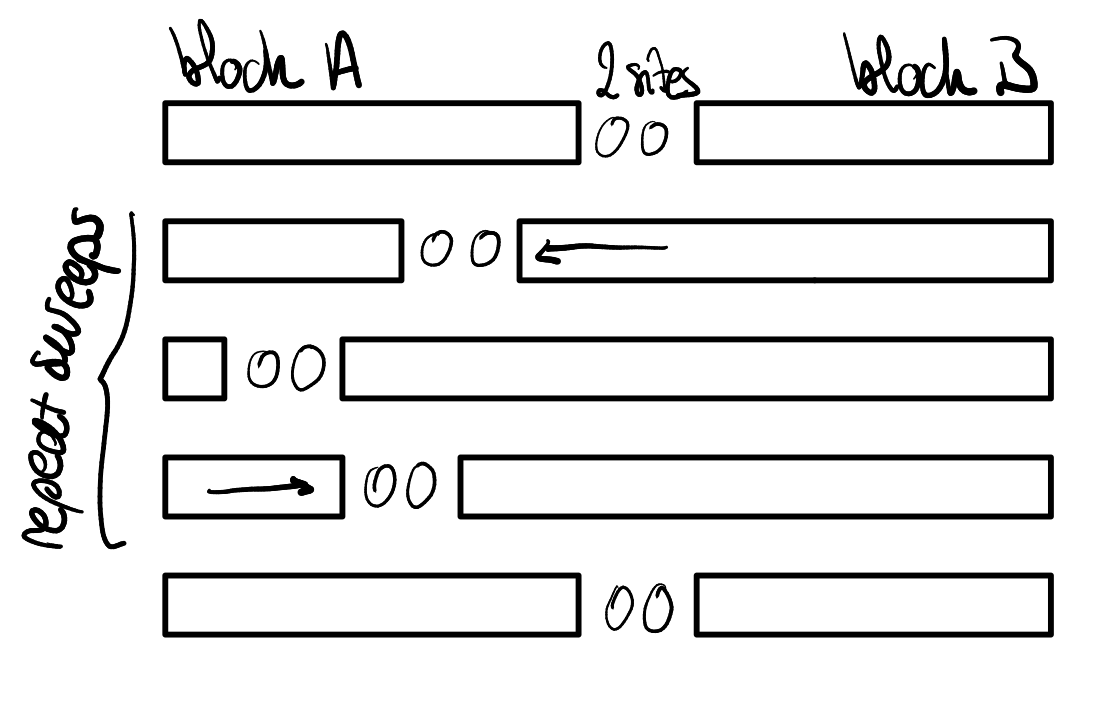
\includegraphics[scale=0.16]{figs/dmrgSweeps.png}
        \end{column}
    \end{columns}
\end{frame}

\begin{frame}
    \frametitle{Results -- Central charge}

    \begin{block}{Transverse-Field Ising}
        \begin{itemize}
            \item TFI model $$\mathcal{H} = -J\sum_i \sigma^x_i \sigma^x_{i+1} - h\sum_i \sigma^z_i$$
            \pause
            \item Described by CFT with central charge $c= \frac{1}{2}$ at criticality $|J| = |h|$
        \end{itemize}
    \end{block}

    \pause
    \begin{block}{Central charge}
        For open boundary conditions, entanglement entropy given by Cardy-Calabrese formula $$S(l) = \frac{c}{6} \ln\left[\frac{2L}{\pi} \sin \frac{\pi l}{L} \right] + \text{const}$$ on bond $l$ (in MPS language) for system of length $L$
    \end{block}
\end{frame}

\begin{frame}
    \frametitle{Results -- Central charge}

    \begin{columns}
        \begin{column}{0.57\linewidth}
            \begin{figure}
                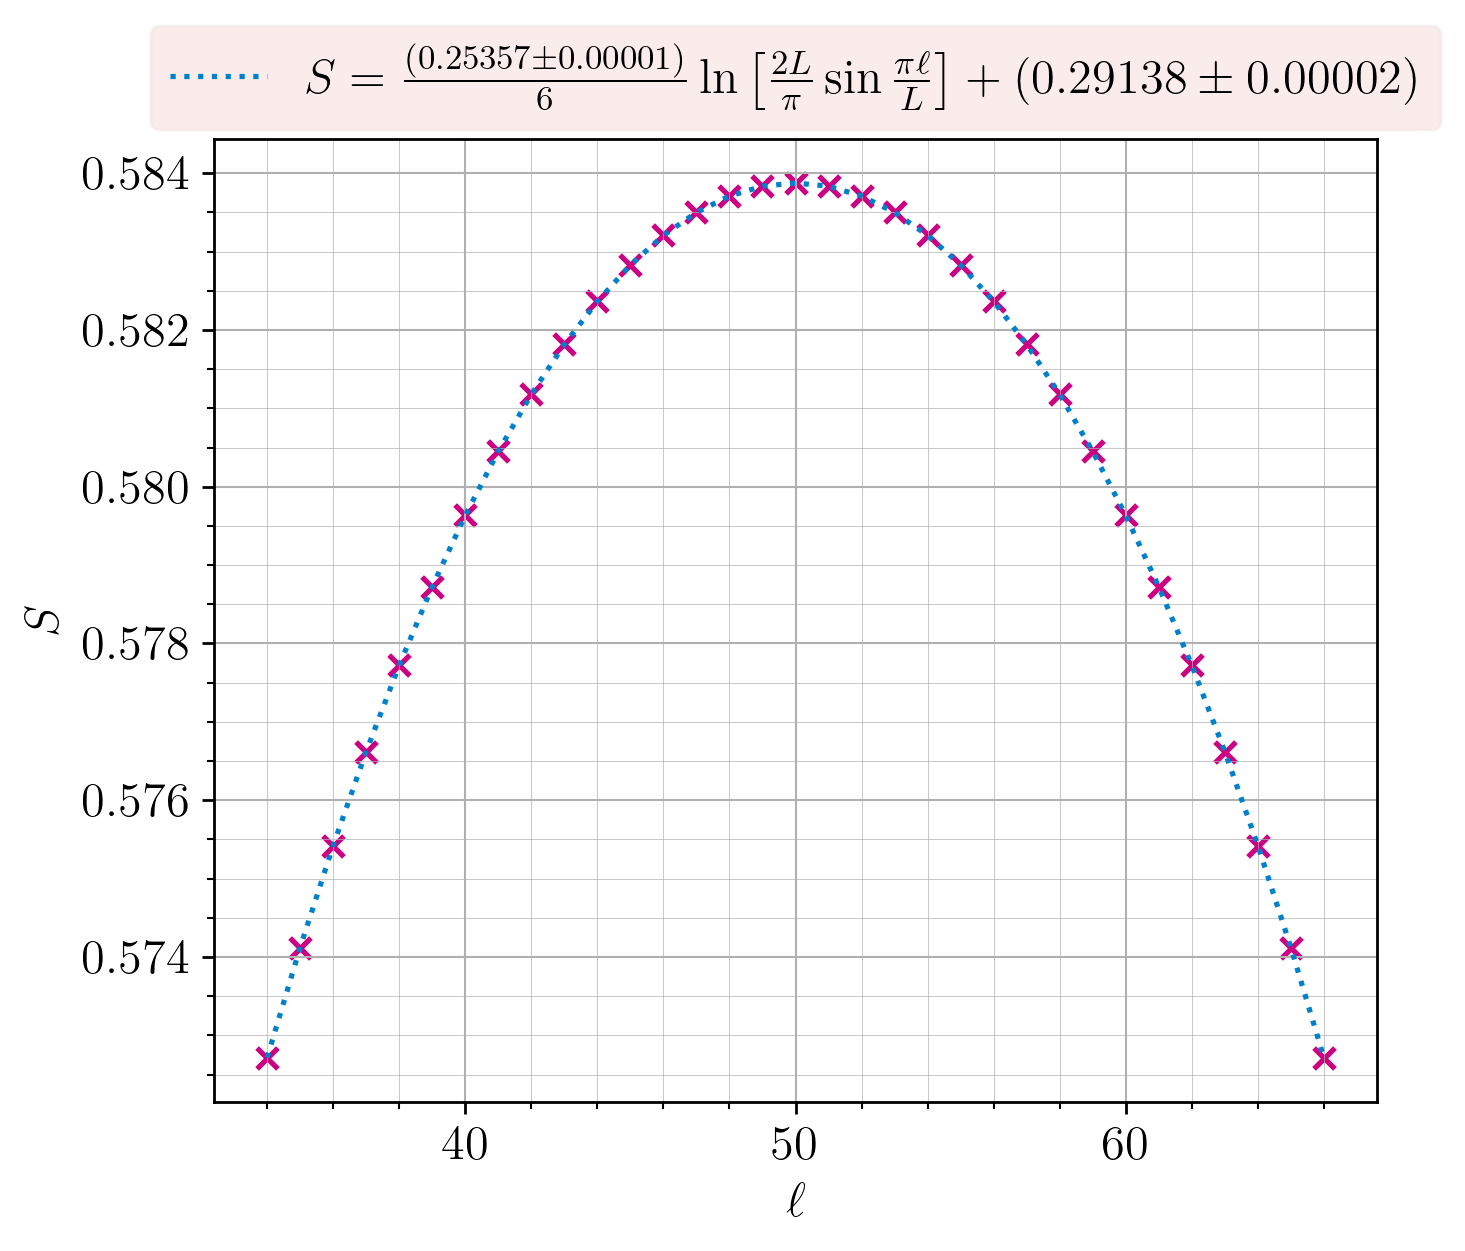
\includegraphics[scale=0.43]{../graphs/entropies/alone_L=100.0_chi=100.0_J=1.0_h=1.0_i=1.0_3=0.0_c=0.0.png}
                \caption{TFI with $J=h$, $L=100$, $\chi=100$}
            \end{figure}
        \end{column}

        \begin{column}{0.6\linewidth}
            \vspace{0.45cm}
            \pause
            \begin{figure}
                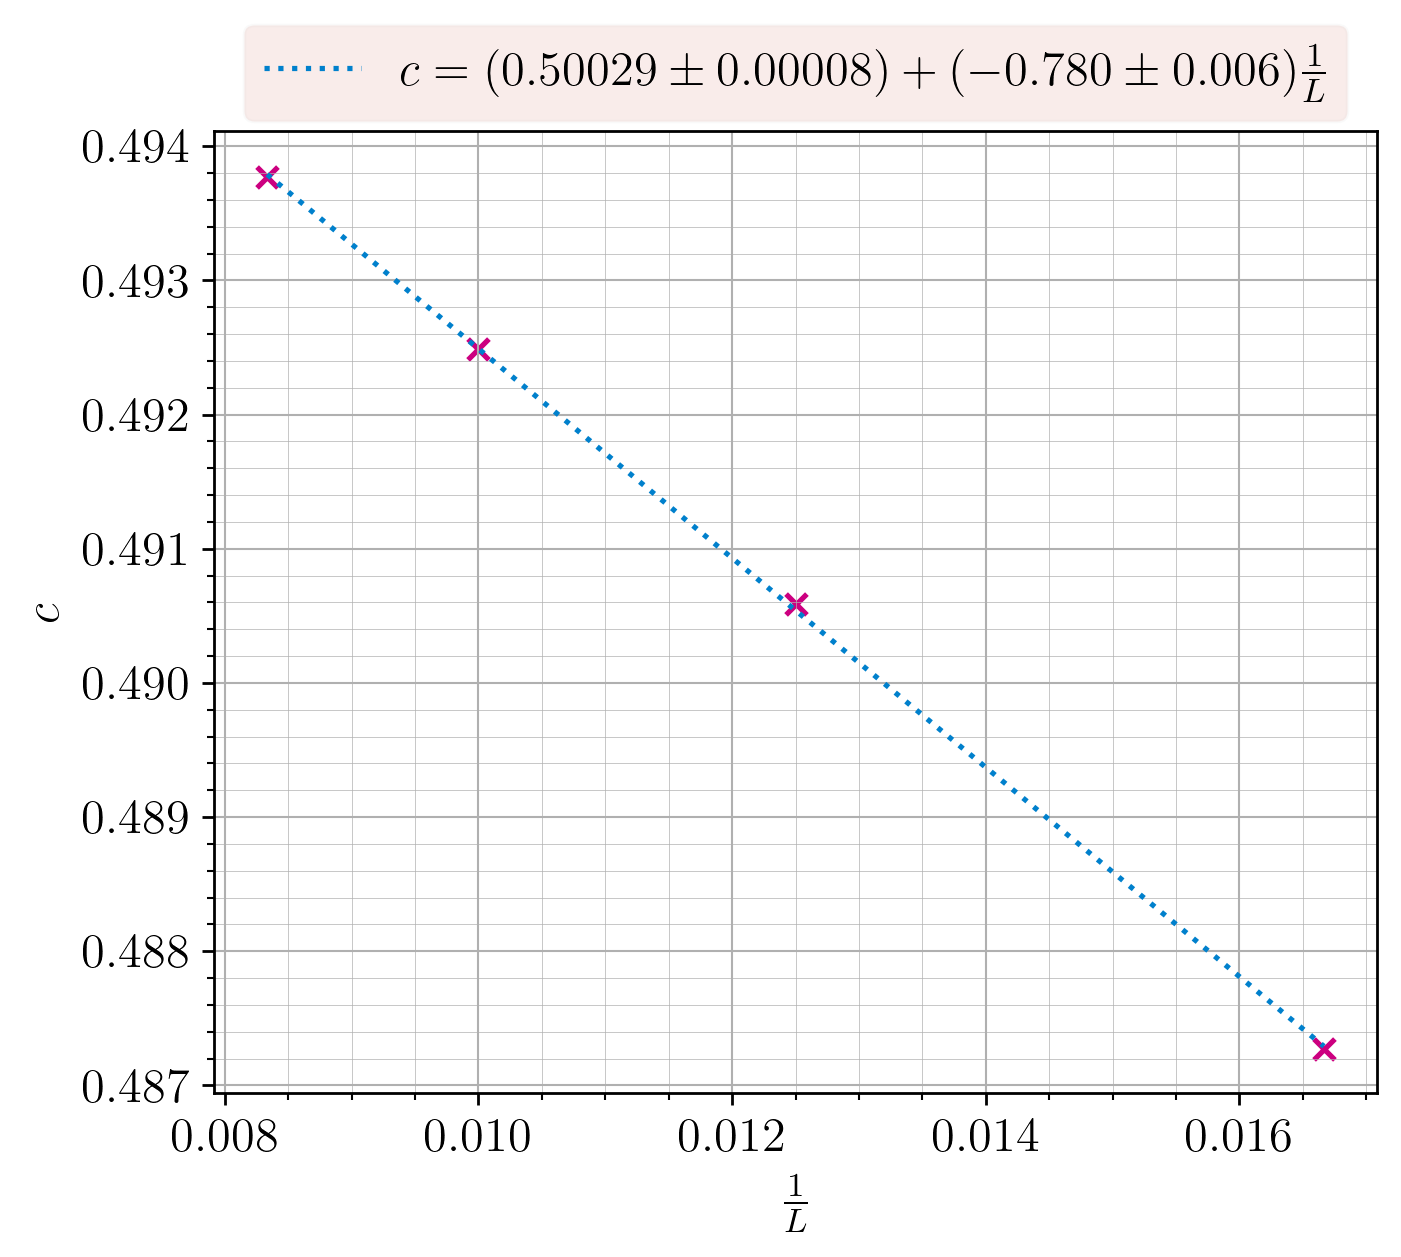
\includegraphics[scale=0.43]{../graphs/entropies/calabrese_chi=100.0_J=1.0_h=1.0_i=1.0_3=0.0_c=0.0.png}
                \caption{TFI with $J=h$, $\chi=100$}
            \end{figure}
        \end{column}        
    \end{columns}
\end{frame}

\begin{frame}
    \frametitle{Results -- Central charge}

    \begin{columns}
        \begin{column}{0.5\linewidth}
            \begin{block}{OF model}
                \begin{itemize}
                    \item is in Ising CFT universality class for $\lambda_3/\lambda_I \in [0, 0.856[ \Rightarrow c=1/2$
                    \pause
                    \item is in TCI CFT universality class for $\lambda_3/\lambda_I \simeq 0.856 \Rightarrow c=7/10$
                    \pause
                    \item is gapped for $\lambda_3/\lambda_I > 0.856 \Rightarrow c=0$
                \end{itemize}
            \end{block}
        \end{column}        

        \begin{column}{0.55\linewidth}
            \pause
            \begin{figure}
                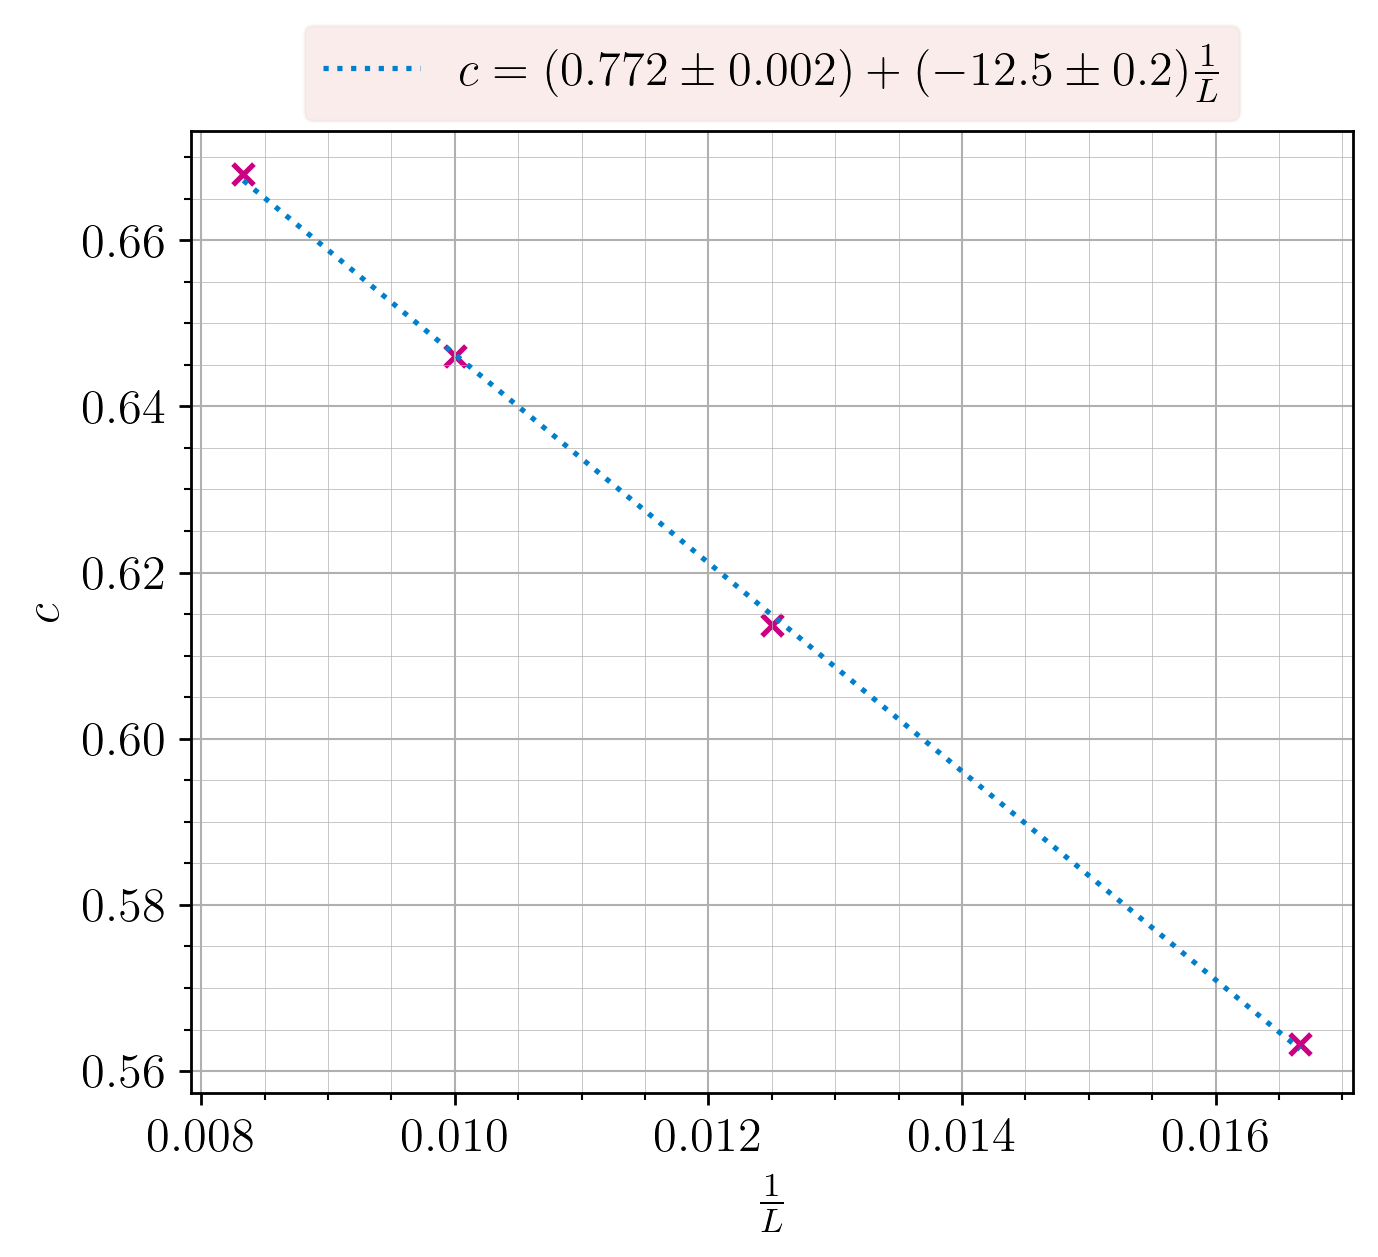
\includegraphics[scale=0.43]{../graphs/entropies/calabrese_chi=100.0_J=1.0_h=1.0_i=1.0_3=0.856_c=0.0.png}
                \caption{OF with $\lambda_3/\lambda_I \simeq 0.856$, $\chi=100$}
            \end{figure}
        \end{column}
    \end{columns}
\end{frame}

\begin{frame}
    \frametitle{Results -- Central charge}

    \begin{columns}
        \begin{column}{0.35\linewidth}
            \begin{block}{Problem}
                \begin{itemize}
                    \item Extrapolates to 0.772 instead of 0.7 !
                    \pause
                    \item Good way to extrapolate ?
                    \pause
                    \item Seems not as we approach $\lambda_3/\lambda_I \simeq 0.856$\\$\rightarrow$ need to go to larger $L$ (difficult)
                \end{itemize}
            \end{block}
        \end{column}        

        \begin{column}{0.75\linewidth}
            \begin{figure}
                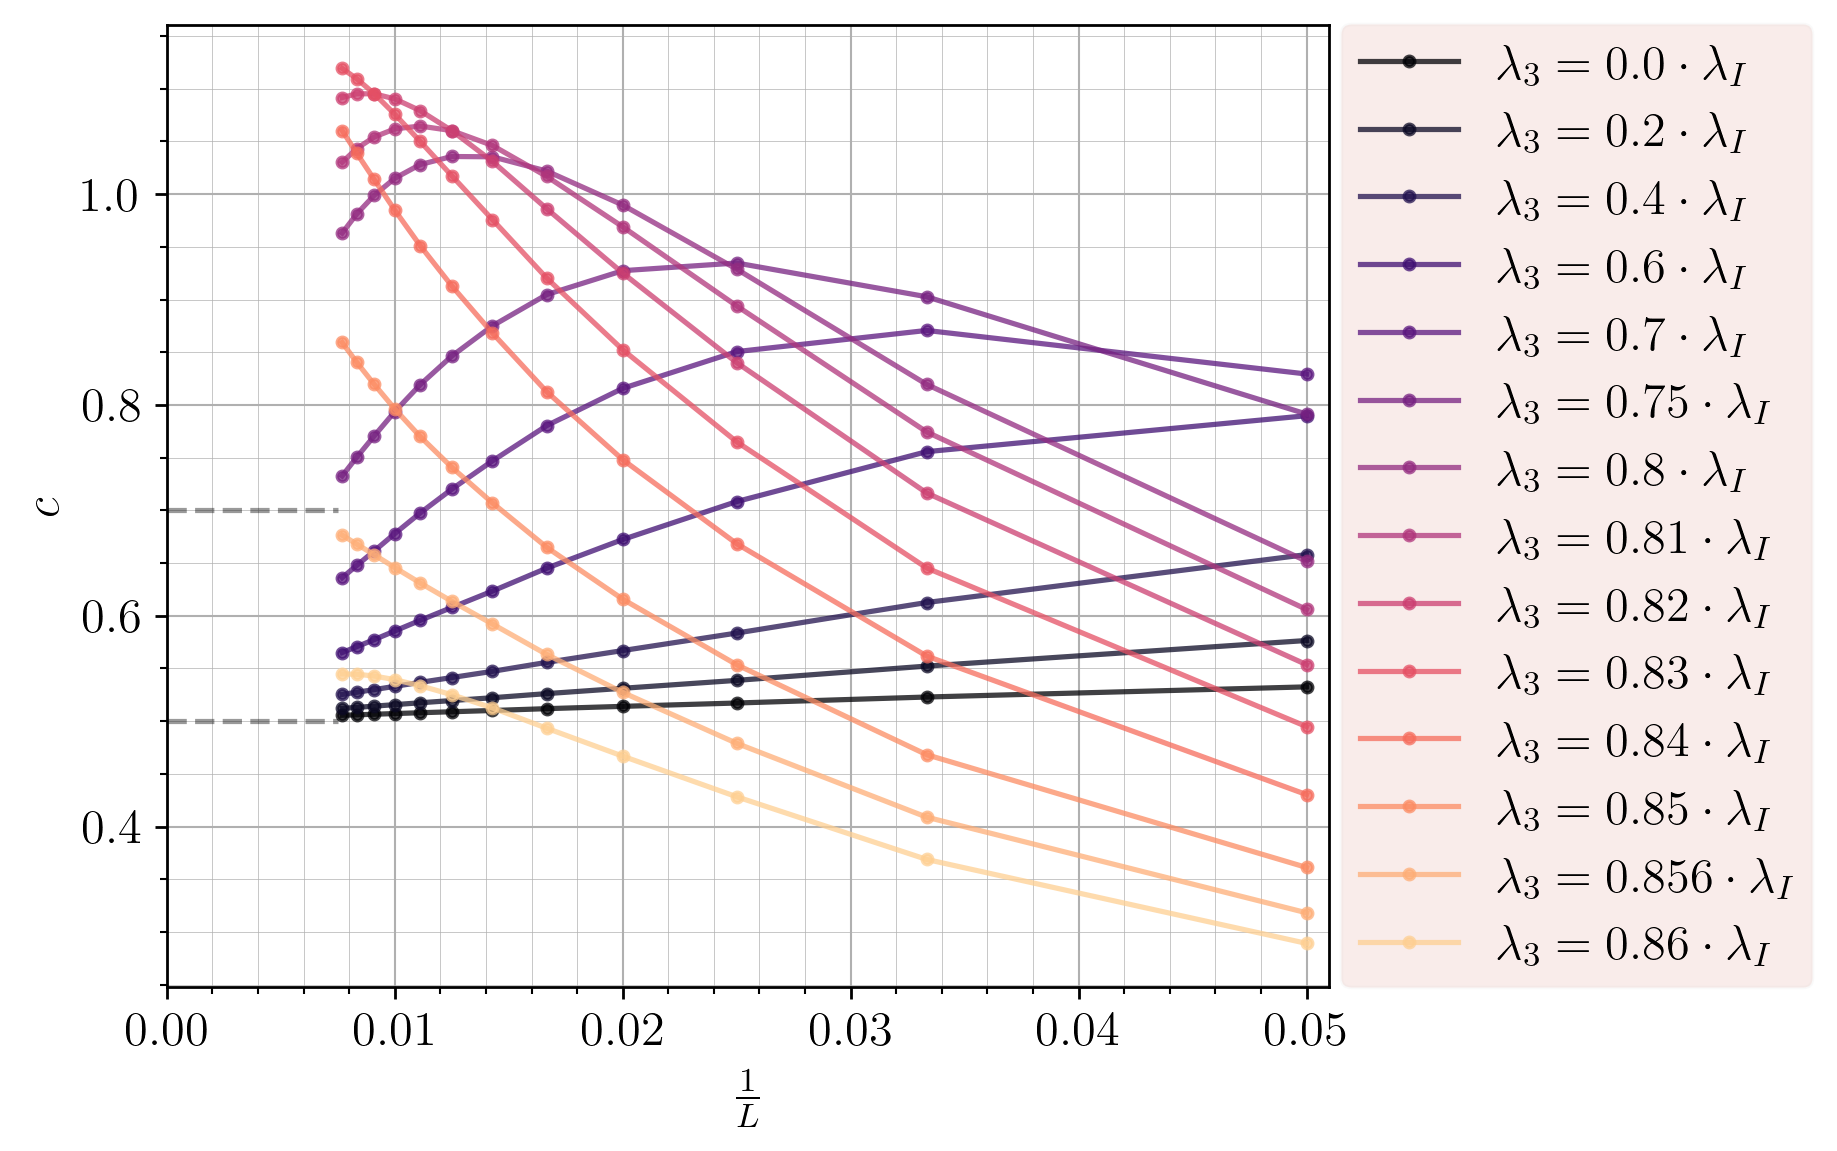
\includegraphics[scale=0.43]{../graphs/phase/chi=100.0_J=1.0_h=1.0_i=1.0_c=0.0.png}
                \caption{OF with $\chi=100$}
            \end{figure}
        \end{column}
    \end{columns}
\end{frame}

\begin{frame}
    \frametitle{Results -- Exicted energies}

    \begin{columns}
        \begin{column}{0.5\linewidth}
            \begin{block}{Compute ratios}
                \begin{itemize}
                    \item Energy ratios universal at critical point described by CFT
                    \pause
                    \item Use them to improve characterization of tricritical point
                \end{itemize}
            \end{block}

            \pause
            \begin{block}{Excited spectrum}
                \begin{itemize}
                    \item Get excited energies directly through diagonalization of the effective Hamiltionian in 2-site update, follow N. Chepiga and F. Mila \href{https://link.aps.org/doi/10.1103/PhysRevB.96.054425}{\color{orange}{Phys. Rev. B \textbf{96}, 054425 (2017)}}
                    \pause
                    \item Works very well for critical TFI (expect slope 2)
                \end{itemize}
            \end{block}
        \end{column}        

        \begin{column}{0.55\linewidth}
            \begin{figure}
                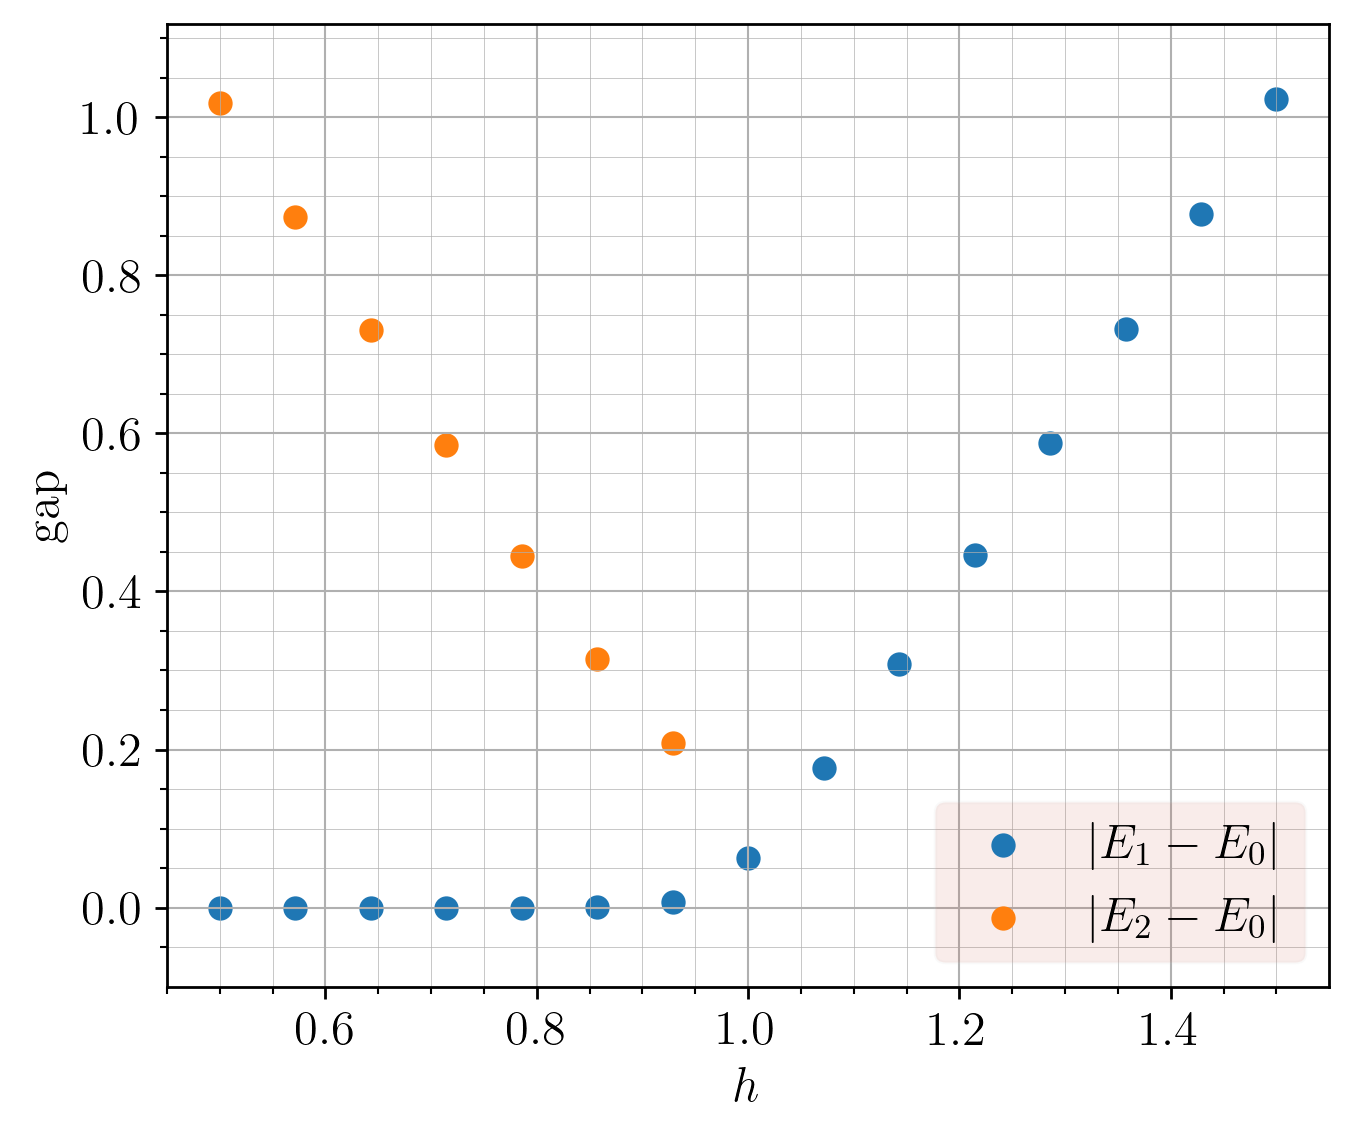
\includegraphics[scale=0.43]{../graphs/transition/gap_L=50_chi=50.0_J=1.0_i=0.5_3=0.0_c=0.0.png}
                \caption{TFI with $J=1$, $L=50$, $\chi=50$}
            \end{figure}
        \end{column}
    \end{columns}
\end{frame}

\begin{frame}
    \frametitle{Conclusion}

    \begin{block}{Periodic boundary conditions}
        \begin{itemize}
            \item However ratios need PBCs energies $$R_1 = \frac{A_0^- - P_0^+}{P_1^+-P_0^+},\ R_2 = \frac{P_0^- - P_0^+}{P_1^+-P_0^+},\ R_3 = \frac{P_1^- - P_0^+}{P_1^+-P_0^+}$$
            \pause
            \item Proving 3-fold degeneracy of ground state at $\lambda_I=\lambda_3$ need PBCs too
            \pause
            \item DMRG with MPS as a loop is not suited (generalized eigenvalue problem + large $\chi$)
            \pause
            \item Can fold MPS and reformulate MPO (finalization...)
        \end{itemize}
    \end{block}

    \vspace{0.5cm}
    \hspace{1cm}
    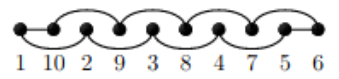
\includegraphics[scale=0.43]{figs/foldedMPS.png}
\end{frame}

\end{document} % --------------------